\documentclass[aspectratio=169]{beamer}
\usepackage{xcolor}
\usepackage{algorithm}
\usepackage{algpseudocode}
\usepackage{listings}
\usepackage{hyperref}
\usepackage{alltt}
\usepackage{mathpartir}
\usepackage{framed}
\usepackage{tikz}
\usepackage{crayola}
\usepackage{multicol}
\usetikzlibrary{positioning,shapes,arrows,backgrounds,fit, calc,automata,shadows}
\usetikzlibrary{decorations, decorations.markings}

\title[Sujit]{A Novel Approach to Automated Evaluation of Programming Assignments}

\author{Sujit Kumar Chakrabarti}
\institute{IIITB}
\date{November 20, 2021}

\logo{\includegraphics[scale=0.1]{/home/sujit/IIITB/misc/iiitbLogo.jpeg}}

\AtBeginSection[]
{
  \begin{frame}<beamer>
    \frametitle{Outline for section \thesection}
    \tableofcontents[currentsection]
  \end{frame}
}

\begin{document}
\maketitle

\definecolor{lightblue}{rgb}{0.8,0.93,1.0} % color values Red, Green, Blue
\definecolor{darkblue}{rgb}{0.4,0.3,1.0} % color values Red, Green, Blue
\definecolor{Blue}{rgb}{0,0,1.0} % color values Red, Green, Blue
\definecolor{darkgreen}{rgb}{0,0.7,0.2} % color values Red, Green, Blue
\definecolor{Red}{rgb}{1,0,0} % color values Red, Green, Blue
\definecolor{Pink}{rgb}{0.7,0,0.2}
\definecolor{links}{HTML}{2A1B81}
\definecolor{mydarkgreen}{HTML}{126215}
\newcommand{\highlight}[1]{{\color{Red}(#1)}}
\newcommand{\comment}[1]{\begin{tiny}
	{\color{blue}(#1)}
	\end{tiny}
}
\newcommand{\keyword}[1]{{\color{mydarkgreen}\textbf{\texttt{#1}}}}
\newcommand{\code}[1]{
	{\color{mydarkgreen}
		\begin{alltt}
			{#1}
		\end{alltt}
	}
}
\newcommand{\myheader}[1]{
	{\color{darkblue}
		\begin{Large}
			\begin{center}
				{#1}
			\end{center}
		\end{Large}
	}
}
\newcommand{\myminorheader}[1]{
	{\color{purple}
		\begin{large}
			{#1}
		\end{large}
	}
}

\newcommand{\myprod}[0]{\hspace{0.5cm}$::=$\hspace{0.5cm}}
\newcommand{\mychoice}[0]{\hspace{0.75cm}$|$\hspace{0.25cm}}

\tikzstyle{bb}=[%
      rectangle, draw=black, thick, fill=OliveGreen!30, drop shadow, align=center,
      text ragged, minimum height=1.0em, minimum width=2em, inner sep=3pt
]

\tikzstyle{inv}=[%
      rectangle, draw=none,  align=center,
      text ragged, minimum height=2em, minimum width=2em, inner sep=6pt
]

\tikzstyle{db}=[%
      ellipse, draw=black, thick, fill=pink, drop shadow, align=center,
      text ragged, minimum height=1.0em, inner sep=3pt
]

\tikzstyle{jn}=[%
      ellipse, draw=black, thick, fill=black, inner sep = 0, outer sep = 0
]

\tikzstyle{io}=[%
      trapezium, trapezium left angle=60, trapezium right angle=120, draw=black, thick, fill=brown, drop shadow,
      text ragged, minimum height=2em, minimum width=2em, inner sep=6pt, align=center
]

\tikzstyle{glio}=[%
      trapezium, trapezium left angle=60, trapezium right angle=120, draw=red, line width = 1mm, fill=brown, drop shadow,
      text ragged, minimum height=2em, minimum width=2em, inner sep=6pt
]
\tikzstyle{gl}=[%
      rectangle, draw=red, line width = 1mm, fill=lightblue, drop shadow,
      text ragged, minimum height=2em, minimum width=2em, inner sep=6pt
]

\tikzstyle{en}=[%
      rectangle, draw=black, thick, fill=none,
      text ragged, minimum height=2em, minimum width=2em, inner sep=6pt
1]

\tikzstyle{sh}=[%
      rectangle, draw=gray, thick, fill=none, color = gray,
      text ragged, minimum height=2em, minimum width=2em, inner sep=6pt
]

\tikzstyle{cfpath}=[->, thick, draw=Black]

\tikzstyle{dfpath}=[->, thick, draw=red]

\tikzstyle{sh2e} = [shift={(0.5,0)}]

\lstset{
	language = Python,
	basicstyle = \ttfamily,
	stringstyle = \ttfamily,
	keywordstyle=\color{Blue}\bfseries,
	identifierstyle=\color{brown},
	commentstyle=\color{darkgreen},
	frameround=tttt,
	mathescape=true,
%	numbers=left
	showstringspaces=false
}
\mathchardef\mhyphen="2D


\lstdefinestyle{pc}{
	language = Python,
	basicstyle = \ttfamily,
	stringstyle = \ttfamily,
	keywordstyle=\color{Blue}\bfseries,
	identifierstyle=\color{Pink},
	commentstyle=\color{darkgreen},
	frameround=tttt,
	frame=single,
%	numbers=left
	mathescape=true,
	showstringspaces=false
}

\lstdefinestyle{jc}{
	language = Java,
	basicstyle = \ttfamily\scriptsize,
	stringstyle = \ttfamily,
	keywordstyle=\color{Blue}\bfseries,
	identifierstyle=\color{Pink},
	commentstyle=\color{darkgreen},
	frameround=tttt,
%	numbers=left
	showstringspaces=false
}

\lstdefinestyle{cc}{
	language = Caml,
	basicstyle = \tiny\ttfamily,
	stringstyle = \color{red}\ttfamily,
	keywordstyle=\color{Blue}\bfseries,
	identifierstyle=\ttfamily,
	frameround=tttt,
	numbers=none,
	showstringspaces=false,
	escapeinside={(*@}{@*)}
}

\lstdefinestyle{oc}{
	language = bash,
	backgroundcolor = \color{black},
	basicstyle = \tiny\ttfamily\color{white},
	stringstyle = \color{red}\ttfamily,
	keywordstyle=\color{white}\bfseries,
	identifierstyle=\ttfamily,
	frameround=tttt,
	numbers=none,
	showstringspaces=false,
	escapeinside={(*@}{@*)}
}


\section{Introduction}

% frame begin %%%%%%%%%%%%%%%%%%%%%%%%
\begin{frame}{Why Automated Evaluation?}

\begin{itemize}
\item Online learning platforms: Coursera, Udacity, EdX ...
\item Online programming contests: ACM ICPC, HakerEarth, HackerRank, CodeChef ...
\pause
\item Introductory programming courses
\pause
\item Error prone, labour intensive, repetitive
\end{itemize}
\end{frame}
% frame end %%%%%%%%%%%%%%%%%%%%%%%%

% frame begin %%%%%%%%%%%%%%%%%%%%%%%%
\begin{frame}[fragile]{Automated Evaluation}

\begin{enumerate}
\item Speed
\item Scalability
\item Objectivity
\item Transparency
\end{enumerate}
\end{frame}
% frame end %%%%%%%%%%%%%%%%%%%%%%%%


\section{AEPA System}
% frame begin %%%%%%%%%%%%%%%%%%%%%%%%
\begin{frame}{Automated Evaluation System}

\begin{itemize}
\item Automatically evaluates programming assignments using testing
\item Several human weeks $\longrightarrow$ a few seconds
\item Has enabled more frequent, deeper formative assessments with shorter feedback cycles
\end{itemize}
\end{frame}
% frame end %%%%%%%%%%%%%%%%%%%%%%%%

% frame begin %%%%%%%%%%%%%%%%%%%%%%%%
\begin{frame}{AEPA Workflow}

\begin{center}
\resizebox{!}{0.75\textheight}{
\begin{tikzpicture}
\node[bb, fill=orange!20](1){Create and publish assignment};
\node[bb, fill=orange!20](2)[below left = 1cm of 1]{Create \\ evaluation \\ script};
\node[bb, fill=green!20](3)[below right = 1cm of 1]{Solve \\ and \\ submit};
\node[bb, fill=orange!20](4)[below = 3cm of 1]{Run evaluation};
\node[bb, fill=orange!20](5)[below = 0.5cm of 4]{Share result and script};
\node[bb, fill=green!20](6)[below =  0.5cm of 5]{Review and feedback};
\node[bb, fill=orange!20](7)[below =  0.5cm of 6]{Update and run};
\node[bb, fill=orange!20](8)[below =  0.5cm of 7]{Publish result};

\draw[->, Red, thick](1) -- (2);
\draw[->, Red, thick](1) -- (3);
\draw[->, Red, thick](2) -- (4);
\draw[->, Red, thick](3) -- (4);
\draw[->, Red, thick](4) -- (5);
\draw[->, Red, thick](5) -- (6);
\draw[->, Red, thick](6) -- (7);
\draw[->, Red, thick](7) -- (8);
\end{tikzpicture}
}
\end{center}
\end{frame}
% frame end %%%%%%%%%%%%%%%%%%%%%%%%


% frame begin %%%%%%%%%%%%%%%%%%%%%%%%
\begin{frame}{Testing}
{A Test Setup}

\begin{center}

\begin{tikzpicture}
\node[inv](i) {$I_i$};
\node[bb, right = of i](th) {Test \\ Harness};
\node[inv, above = of th](put) {Program \\ under \\ Test};
\node[circle, draw=black, right = of th](cmp) {};
\draw[-] (cmp.south west) to (cmp.north east);
\draw[-] (cmp.south east) to (cmp.north west);
\node[inv, above = of cmp](e) {$E_i$};
\node[inv, right = of cmp](res) {$R_i$ (Pass/Fail)};

\draw[-latex] (i) to (th);
\draw[-latex] (put) to (th);
\draw[-latex] (th) to node[above]{$O_i$}(cmp);
\draw[-latex] (e) to (cmp);
\draw[-latex] (cmp) to (res);

\end{tikzpicture}
\begin{multicols}{2}
\begin{tabular}{| c | c |}
\hline
$I_i$ & Test input \\
\hline
$E_i$ & Expected output \\
\hline
$O_i$ & Actual output \\
\hline
$R_i$ & Test result \\
\hline
\end{tabular}

\myminorheader{Assigning Marks:}
\begin{equation*}
M = \sum k_i R_i
\end{equation*}
\end{multicols}
\end{center}

\end{frame}
% frame end %%%%%%%%%%%%%%%%%%%%%%%%

% frame begin %%%%%%%%%%%%%%%%%%%%%%%%
\begin{frame}{AEPA Artefacts}

\begin{center}
\resizebox{0.6\textwidth}{!}{
\begin{tikzpicture}
\node[bb](ev){Test\\code};

\node[bb, above right=2cm of ev](ms){Model \\ Solution};

\node[bb, below right=2cm of ev](ss){Submitted \\ Solution};

\draw[->] (ev) -- + (0:1.5) |- node[left, align=center]{
\includegraphics[scale=0.4]{images/doc.png} \\ \begin{scriptsize}test input\end{scriptsize}}(ms);

\draw[->] (ev) -- + (0:1.5) |- node[left, align=center]{
\includegraphics[scale=0.4]{images/doc.png} \\ \begin{scriptsize}test input\end{scriptsize}}(ss);

\pause
\node[inv, right=of ms] (eo){
\includegraphics[scale=0.4]{images/doc.png}};
\node[inv, right=0.1cm of eo] (eolabel){Expected \\ output};

\node[inv, right= of ss] (ao){
\includegraphics[scale=0.4]{images/doc.png}};
\node[inv, right=0.1cm of ao] (aolabel){Actual \\ output};

\draw[->](ms) -- (eo);
\draw[->](ss) -- (ao);

\pause
\node[circle, draw=black, below = 1.5cm of eo](cmp) {};
\draw[-] (cmp.south west) to (cmp.north east);
\draw[-] (cmp.south east) to (cmp.north west);

\draw[<-, dashed] (cmp) -- + (-1, 0) -| (ev.east);
\draw[->, dashed] (eo) -- (cmp);
\draw[->, dashed] (ao) -- (cmp);

\pause
\node[inv, right = of cmp](res) {Result};

\draw[->](cmp) -- (res);
\end{tikzpicture}
}
\end{center}
\end{frame}
% frame end %%%%%%%%%%%%%%%%%%%%%%%%

% frame begin %%%%%%%%%%%%%%%%%%%%%%%%
\begin{frame}{Design}
{System Architecture}
\begin{center}
\resizebox{!}{0.8\textheight}{
\begin{tikzpicture}
\node[bb](ev){Evaluator};

\node[bb, fill=Red!20, above left= 0.2cm of ev, yshift=1cm](ts1){Test \\ suite 1};
\draw[->, thick, BrickRed](ev) |- node[left, near start] {\rotatebox{90}{$\rightarrow W_1$}} node[above, near end] {$\rightarrow\eta_1$}(ts1);
\node[bb, fill=Red!20, below left= 0.2cm of ev, yshift=-1cm](tsn){Test \\ suite $n$};
\draw[->, thick, BrickRed](ev) |- node[above left] {\rotatebox{90}{$W_n\ \leftarrow $}} node[below, near end]{$\rightarrow\eta_n$}(tsn);

\node[bb, fill=Blue!20, above left= 0.2cm of ts1, xshift=-1cm](tc11){Test \\ case 1.1};
\draw[->, thick, BrickRed](ts1) |- node[below, near end] {$ w_{1.1} \leftarrow$} node[above, near end] {$\rightarrow M_{1.1}$}(tc11);

\node[inv, left= 1.5cm of ts1](dots2){\rotatebox{90}{...}};

\node[bb, fill=Blue!20, below left= 0.2cm of ts1, xshift=-1cm](tc1n){Test \\ case $1.m_1$};
\draw[->, thick, BrickRed](ts1) |- node[below, near end] {$w_{1.m_1} \leftarrow$} node[above, near end] {$\rightarrow M_{1.m_1}$} (tc1n);

\node[bb, fill=Blue!20, above left= 0.2cm of tsn, xshift=-1cm](tcm1){Test \\ case $n.1$};
\draw[->, thick, BrickRed](tsn) |- node[below, near end] {$ w_{n.1} \leftarrow$} node[above, near end] {$\rightarrow M_{n.1}$} (tcm1);

\node[inv, left= 1.5cm of tsn](dots3){\rotatebox{90}{...}};

\node[bb, fill=Blue!20, below left= 0.2cm of tsn, xshift=-1cm](tcmn){Test \\ case $n.m_n$};
\draw[->, thick, BrickRed](tsn) |- node[below, near end] {$w_{n.m_n} \leftarrow$} node[above, near end] {$\rightarrow M_{n.m_n}$} (tcmn);

\node[inv, left= 0.2cm of ev](dots4){\rotatebox{90}{...}};


\end{tikzpicture}
}
\end{center}
\begin{center}
\end{center}
\end{frame}
% frame end %%%%%%%%%%%%%%%%%%%%%%%%

% frame begin %%%%%%%%%%%%%%%%%%%%%%%%
\begin{frame}{Design}
{Types of Programs}
\begin{itemize}
\item Programs with input/output
\item Programs using/computing values
\item Functions returning values
\item Functions with input/output
\item Questions about structural properties
\end{itemize}
\end{frame}
% frame end %%%%%%%%%%%%%%%%%%%%%%%%

% frame begin %%%%%%%%%%%%%%%%%%%%%%%%
\begin{frame}{Design}
{\lstinline@evaluate.py@ API\footnote{https://github.com/sujitkc/evaluate/}}
\begin{itemize}
\item \lstinline@equals@
\item \lstinline@eval_matfun@
\item \lstinline@eval_named_proc_1@
\item \lstinline@eval_named_proc_2@
\item \lstinline@eval_f_calls_g@
\item \lstinline@is_recursive@
\item \lstinline@is_inner_function@
\item \lstinline@num_of_classdefs@
\item \lstinline@num_of_classdefs@
\end{itemize}
\end{frame}
% frame end %%%%%%%%%%%%%%%%%%%%%%%%

% frame begin %%%%%%%%%%%%%%%%%%%%%%%%
\begin{frame}{Design}
{Dealing with Infinite Loops -- Failing Tests}
\pause
\begin{center}
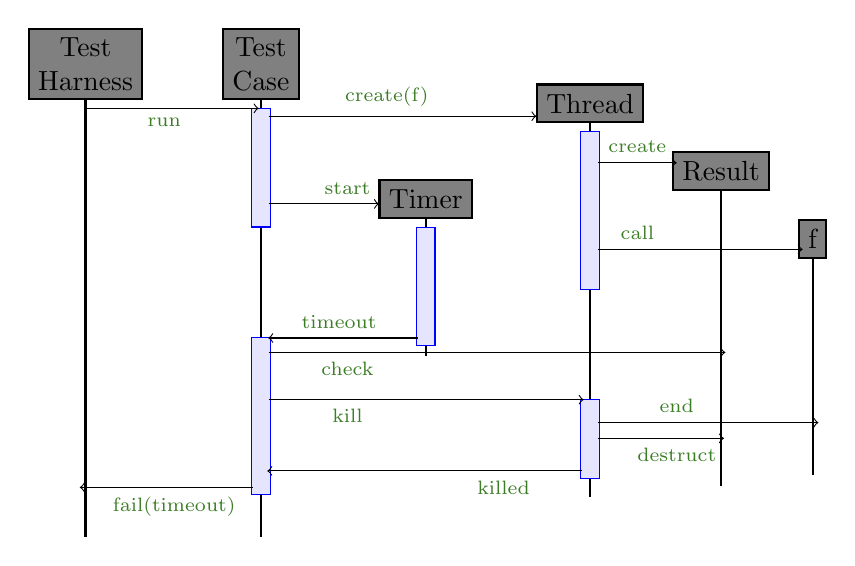
\begin{tikzpicture}
\node[rectangle, draw=black, thick, fill=Gray, align=center](th){Test \\ Harness};
\draw[-, thick](th) --++(-90:6);

\node[rectangle, draw=black, thick, fill=Gray, align=center, right = of th](tc){Test \\ Case};
\draw[-, thick](tc) --++(-90:6);
\node[rectangle, draw = blue, fill = blue!10, minimum width = 0.1cm, minimum height = 1.5cm, below = 0.1cm of tc](tltc1){};
\node[rectangle, draw = blue, fill = blue!10, minimum width = 0.1cm, minimum height = 2cm, below = 3cm of tc](tltc2){};

\node[rectangle, draw=black, thick, fill=Gray, align=center, below right = of tc](timer){Timer};
\draw[-, thick](timer) --++(-90:2);
\node[rectangle, draw = blue, fill = blue!10, minimum width = 0.1cm, minimum height = 1.5cm, below = 0.1cm of timer](tltimer){};

\node[rectangle, draw=black, thick, fill=Gray, align=center, right = 3 cm of tc, yshift = -0.5cm](thread){Thread};
\draw[-, thick](thread) --++(-90:5);
\node[rectangle, draw = blue, fill = blue!10, minimum width = 0.1cm, minimum height = 2cm, below = 0.1cm of thread](tlthread1){};
\node[rectangle, draw = blue, fill = blue!10, minimum width = 0.1cm, minimum height = 1cm, below = 3.5cm of thread](tlthread2){};

\node[rectangle, draw=black, thick, fill=Gray, align=center, below right = 0.5cm of thread](res){Result};
\draw[-, thick](res) --++(-90:4);

\node[rectangle, draw=black, thick, fill=Gray, align=center, below right = 0.5cm of res](f){f};
\draw[-, thick](f) --++(-90:3);

\pause
\draw[->]($(th.south) + (0,-0.1)$) node[below, xshift = 1cm]{\color{OliveGreen}\scriptsize run} --++(0:2.2);
\pause
\draw[->]($(tc.south) + (0.1,-0.2)$) node[above, xshift = 1.5cm]{\color{OliveGreen}\scriptsize create(f)} --++(0:3.4);
\pause
\draw[->]($(tlthread1.north) + (0.1,-0.4)$) node[above, xshift = 0.5cm]{\color{OliveGreen}\scriptsize create} --++(0:1);
\draw[->]($(tlthread1.north) + (0.1,-1.5)$) node[above, xshift = 0.5cm]{\color{OliveGreen}\scriptsize call} --++(0:2.6);
\pause
\draw[->]($(tltc1.south) + (0.1,0.3)$) node[above, xshift = 1cm]{\color{OliveGreen}\scriptsize start} --++(0:1.4);
\pause
\draw[->]($(tltimer.south) + (-0.1,0.1)$)node[above, xshift = -1cm]{\color{OliveGreen}\scriptsize timeout}  --++(180:1.9);
\pause
\draw[->]($(tltc2.north) + (0.1,-0.2)$) node[below, xshift = 1cm]{\color{OliveGreen}\scriptsize check} --++(0:5.8);
\pause
\draw[->]($(tltc2.north) + (0.1,-0.8)$) node[below, xshift = 1cm]{\color{OliveGreen}\scriptsize kill} --++(0:4);
\pause
\draw[->]($(tlthread2.north) + (0.1,-0.3)$) node[above, xshift = 1cm]{\color{OliveGreen}\scriptsize end} --++(0:2.8);
\pause
\draw[->]($(tlthread2.north) + (0.1,-0.5)$) node[below, xshift = 1cm]{\color{OliveGreen}\scriptsize destruct} --++(0:1.6);
\pause
\draw[->]($(tlthread2.south) + (-0.1,0.1)$) node[below, xshift = -1cm]{\color{OliveGreen}\scriptsize killed} --++(180:4);
\pause
\draw[->]($(tltc2.south) + (-0.1,0.1)$) node[below, xshift = -1cm]{\color{OliveGreen}\scriptsize fail(timeout)} --++(180:2.2);
\end{tikzpicture}
\end{center}
\end{frame}
% frame end %%%%%%%%%%%%%%%%%%%%%%%%

% frame begin %%%%%%%%%%%%%%%%%%%%%%%%
\begin{frame}{Design}
{Dealing with Infinite Loops -- Succeeding Tests}
\pause
\begin{center}
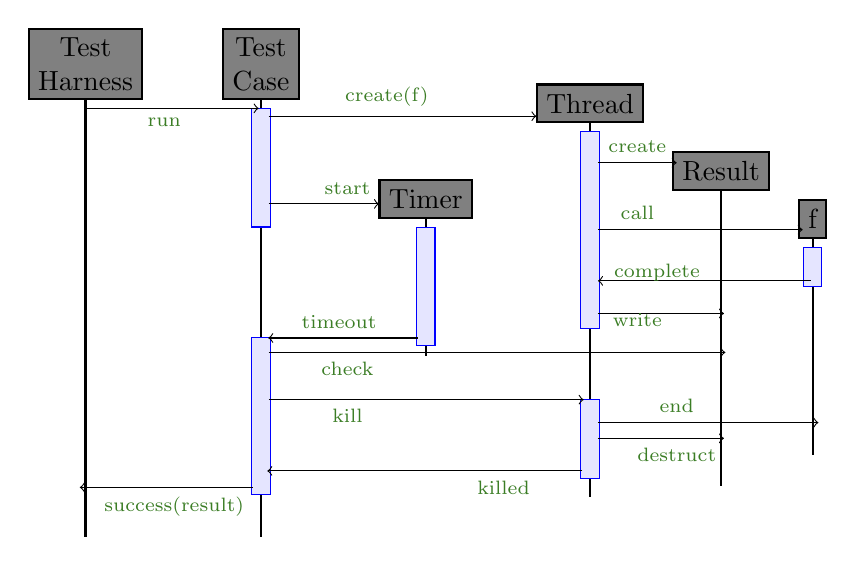
\begin{tikzpicture}
\node[rectangle, draw=black, thick, fill=Gray, align=center](th){Test \\ Harness};
\draw[-, thick](th) --++(-90:6);

\node[rectangle, draw=black, thick, fill=Gray, align=center, right = of th](tc){Test \\ Case};
\draw[-, thick](tc) --++(-90:6);
\node[rectangle, draw = blue, fill = blue!10, minimum width = 0.1cm, minimum height = 1.5cm, below = 0.1cm of tc](tltc1){};
\node[rectangle, draw = blue, fill = blue!10, minimum width = 0.1cm, minimum height = 2cm, below = 3cm of tc](tltc2){};

\node[rectangle, draw=black, thick, fill=Gray, align=center, below right = of tc](timer){Timer};
\draw[-, thick](timer) --++(-90:2);
\node[rectangle, draw = blue, fill = blue!10, minimum width = 0.1cm, minimum height = 1.5cm, below = 0.1cm of timer](tltimer){};

\node[rectangle, draw=black, thick, fill=Gray, align=center, right = 3 cm of tc, yshift = -0.5cm](thread){Thread};
\draw[-, thick](thread) --++(-90:5);
\node[rectangle, draw = blue, fill = blue!10, minimum width = 0.1cm, minimum height = 2.5cm, below = 0.1cm of thread](tlthread1){};
\node[rectangle, draw = blue, fill = blue!10, minimum width = 0.1cm, minimum height = 1cm, below = 3.5cm of thread](tlthread2){};

\node[rectangle, draw=black, thick, fill=Gray, align=center, below right = 0.5cm of thread](res){Result};
\draw[-, thick](res) --++(-90:4);

\node[rectangle, draw=black, thick, fill=Gray, align=center, below right = 0.5cm of res, yshift = 0.25cm](f){f};
\draw[-, thick](f) --++(-90:3);
\node[rectangle, draw = blue, fill = blue!10, minimum width = 0.1cm, minimum height = 0.5cm, below = 0.1cm of f](tlf){};

\pause
\draw[->]($(th.south) + (0,-0.1)$) node[below, xshift = 1cm]{\color{OliveGreen}\scriptsize run} --++(0:2.2);
\pause
\draw[->]($(tc.south) + (0.1,-0.2)$) node[above, xshift = 1.5cm]{\color{OliveGreen}\scriptsize create(f)} --++(0:3.4);
\pause
\draw[->]($(tlthread1.north) + (0.1,-0.4)$) node[above, xshift = 0.5cm]{\color{OliveGreen}\scriptsize create} --++(0:1);
\pause
\draw[->]($(tlthread1.north) + (0.1,-1.25)$) node[above, xshift = 0.5cm]{\color{OliveGreen}\scriptsize call} --++(0:2.6);
\pause
\draw[<-]($(tlthread1.north) + (0.1,-1.9)$) node[above, inner sep=0, outer sep=0, xshift = 0.75cm]{\color{OliveGreen}\scriptsize complete} --++(0:2.7);
\pause
\draw[->]($(tlthread1.south) + (0.1,0.2)$) node[below, , inner sep=0, outer sep=0, xshift = 0.5cm]{\color{OliveGreen}\scriptsize write} --++(0:1.6);

\pause
\draw[->]($(tltc1.south) + (0.1,0.3)$) node[above, xshift = 1cm]{\color{OliveGreen}\scriptsize start} --++(0:1.4);
\pause
\draw[->]($(tltimer.south) + (-0.1,0.1)$)node[above, xshift = -1cm]{\color{OliveGreen}\scriptsize timeout}  --++(180:1.9);
\pause
\draw[->]($(tltc2.north) + (0.1,-0.2)$) node[below, xshift = 1cm]{\color{OliveGreen}\scriptsize check} --++(0:5.8);
\pause
\draw[->]($(tltc2.north) + (0.1,-0.8)$) node[below, xshift = 1cm]{\color{OliveGreen}\scriptsize kill} --++(0:4);
\pause
\draw[->]($(tlthread2.north) + (0.1,-0.3)$) node[above, xshift = 1cm]{\color{OliveGreen}\scriptsize end} --++(0:2.8);
\draw[->]($(tlthread2.north) + (0.1,-0.5)$) node[below, xshift = 1cm]{\color{OliveGreen}\scriptsize destruct} --++(0:1.6);
\pause
\draw[->]($(tlthread2.south) + (-0.1,0.1)$) node[below, xshift = -1cm]{\color{OliveGreen}\scriptsize killed} --++(180:4);
\pause
\draw[->]($(tltc2.south) + (-0.1,0.1)$) node[below, xshift = -1cm]{\color{OliveGreen}\scriptsize success(result)} --++(180:2.2);
\end{tikzpicture}
\end{center}
\end{frame}
% frame end %%%%%%%%%%%%%%%%%%%%%%%%


% frame begin %%%%%%%%%%%%%%%%%%%%%%%%
\begin{frame}{Experience}
{Advantages}
\begin{itemize}
\item Simple setup
\item Simple use
\item Language independence. \emph{The system has already been used by us in two flavours: Python and OCaml.}
\item Data availability. \emph{Extensively used by us for our other related research work.}
\item Transparency
\item Crowdsourced debugging
\item Teaching by example
\end{itemize}
\end{frame}
% frame end %%%%%%%%%%%%%%%%%%%%%%%%

% frame begin %%%%%%%%%%%%%%%%%%%%%%%%
\begin{frame}{Demo}
{Goal}
\begin{itemize}
\item Showcase to intructors of programming (intensive) courses
\item Seek feedback -- features, usability
\end{itemize}
\end{frame}
% frame end %%%%%%%%%%%%%%%%%%%%%%%%

% frame begin %%%%%%%%%%%%%%%%%%%%%%%%
\begin{frame}{Demo}
{Goal}
\begin{scriptsize}

\begin{itemize}
\item Test case
\item Test suite
\item Running an individual test suite: \lstinline@eval_mathop.py@
\item Running all the test suites: \lstinline@eval_all.py@
\item Evaluating all the submissions: \lstinline@eval_all_rollnums.sh@
\item \lstinline@evaluate.py@ library
\item Sharing feedback with the class: \lstinline@pack.sh@ and \lstinline@send-reports.sh@
\end{itemize}
\end{scriptsize}
\end{frame}
% frame end %%%%%%%%%%%%%%%%%%%%%%%%



\end{document}
